\chapter{Pengenalan I : Algoritma}\label{ch:pengantarAlgoritma}

%
- Pengantar
- Permasalahan
- Algoritma
- Peran Pemrograman Pada ALgoritma
- Konsep Algorima dan Pemrograman Dasar
/// PENGAYAAN
- Kontes
%

\section{Pengantar}

\begin{figure}
\centering
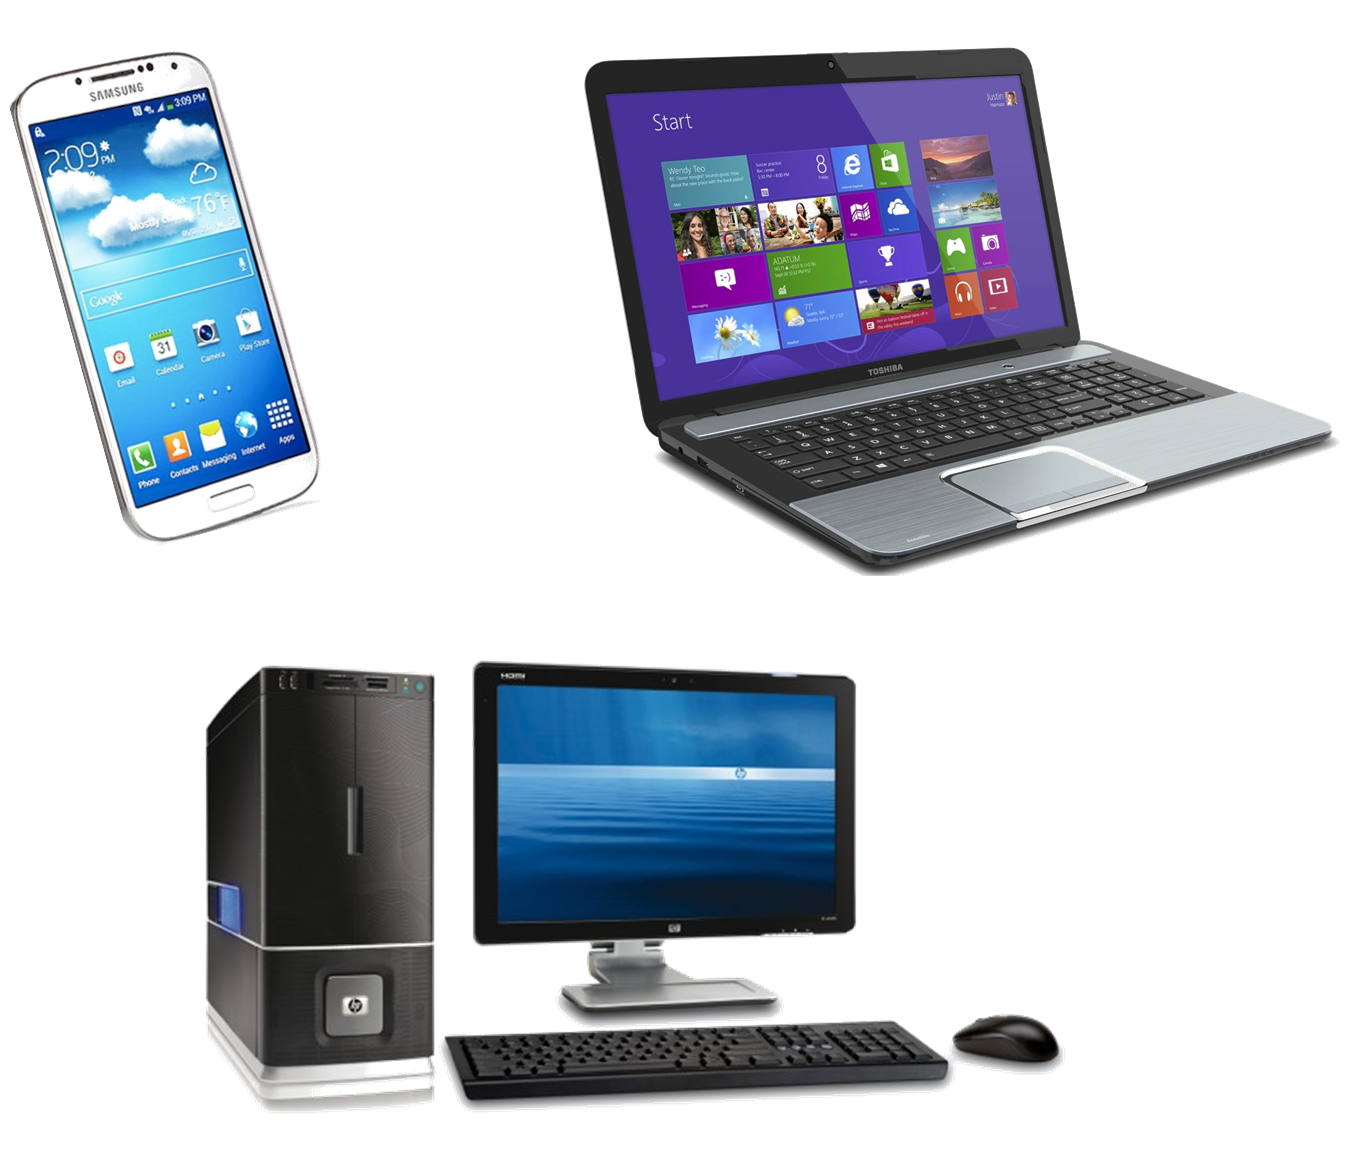
\includegraphics[scale=0.3]{fig/1/Gambar1.png}	
\end{figure}

Teknologi Informasi semakin berkembang pesat setiap saat, hal tersebut bisa dilihat dari munculnya perangkat-perangkat keras seperti \textit{smart phone}, PC, \textit{notebook} dan gadget lainnya. Perangkat-perangkat tersebut tidak berguna tanpa adanya berbagai perangkat lunak (aplikasi) yang berjalan di dalamnya. Perangkat-perangkat lunak tersebut terdiri dari berbagai jenis, antara lain: Sistem Operasi yang merupakan fondasi dari aplikasi-aplikasi lain yang berjalan di atasnya serta perangkat lunak perkantoran seperti \textit{text processor} atau \textit{spreadsheet}, kalender, reminder, penghemat baterai, penghapus berkas tidak berguna dan lain-lain. 
 
Kita sebagai pengguna terkadang hanya mengunduh aplikasi tersebut dari Internet dan menggunakannya tanpa berpikir, bagaimana sebenarnya aplikasi itu dibangun oleh pengembangnya. Sebagai mahasiswa Teknik Informatika, tentunya kita harus tahu lebih banyak daripada seorang pengguna awam. 

Jika dilihat dari sudut pandang tertentu, sebuah aplikasi pada dasarnya dibuat untuk menyelesaikan masalah. Kita ambil sebuah contoh misalnya, sebuah aplikasi \textit{spreadsheet} yang sudah sering kita gunakan yaitu \textit{Microsoft Excel}. Aplikasi ini dapat menyelesaikan banyak masalah mulai dari masalah perhitungan sederhana, logika, statistik, sampai pada pembuatan laporan keuangan yang kompleks. Contoh lain adalah aplikasi permainan yaitu: Poker. Apakah ada masalah yang diselesaikan oleh aplikasi permainan Poker? Ternyata, walaupun aplikasi Poker hanya merupakan aplikasi permainan, akan tetapi dibalik aplikasi tersebut banyak masalah-masalah yang harus diselesaikan agar dapat dinikmati seperti misalnya: proses pengacakan kartu, pembagian kartu, pengecekan kemenangan kartu, serta bagaimana agar pihak komputer (AI) lebih mahir bermain daripada \textit{player}. Poker tentu tidak akan menyenangkan jika ternyata pada pembagian kartu, terdapat kartu yang berulang, proses pembagian kartu yang tidak acak/berulang-ulang, dan pembayaran hadiah kemenangan yang salah. Kesimpulannya, untuk mengembangkan sebuah aplikasi yang bagus diperlukan banyak proses pemecahan masalah didalam aplikasi tersebut.

Dari narasi di atas, muncul pertanyaan seperti:
\begin{enumerate}
	\item Bagaimana perangkat lunak dapat menyelesaikan masalah?
	\item Apakah ada sebuah entitas cerdas di dalamnya yang menyelesaikan masalah dan beradaptasi pada setiap permintaan-permintaan pengguna?
\end{enumerate}
  
Jawaban dari pertanyaan tersebut berkaitan dengan bagian dari perangkat lunak yaitu algoritma. Kita ambil contoh, misalnya pada program \textit{Microsoft Excel}, proses penggunaan rumus-rumus memiliki algoritmanya sendiri, proses membuatan laporan memiliki algoritmanya sendiri dan seterusnya. Demikian juga pada aplikasi permainan Poker, proses pengacakan memiliki algoritmanya sendiri, proses pengecekan kemenangan memiliki algoritmanya sendiri dan seterusnya. Sampai disini kita tahu bahwa, sebuah perangkat lunak selain menyelesaikan banyak masalah juga terdiri dari banyak algoritma (jika masalah yang diselesaikan semakin banyak) dan algoritma adalah sesuatu yang digunakan untuk menyelesaikan masalah.



\section{Masalah}
Sebelum kita membahas lebih lanjut mengenai algoritma, alangkah baiknya kita menelaah mengenai masalah terlebih dahulu. Jika sebelumnya diceritakan mengenai masalah dari sisi perangkat lunak, pada bab ini kita akan melihat masalah pada kehidupan sehari -hari. Coba perhatikan berbagai masalah kehidupan sehari-hari berikut ini:

\begin{enumerate}
	\item Anda diminta untuk menyusun voucher-voucher berikut ini menjadi terurut, sehingga pihak panitia akan mudah melakukan tracking terhadap voucher yang sudah masuk.  
	
	
\begin{center} \Large
  \begin{tabular}[h!]{| c | c | c | c | c | c | c | c | c | c | }
	\hline
    10 & 3 & 8 & 5 & 9 & 2 & 1 &  7 & 4 & 6 \\
	\hline
  \end{tabular}
\end{center}


	\item Anda diminta untuk mencari apakah NIM 141112020 merupakan peserta ujian ? 
		\newpage \Large
			\begin{center}
				\begin{tabular}[h!]{| c | c |}
				\hline
				\multicolumn{2}{|c|}{\textit{PESERTA UJIAN}} \\
				\hline	
				\textit{NIM} & \textit{Nama} \\ \hline
				141110001 & Amir \\ \hline
				141110003 & Budi \\ \hline
				141111111 & Charlie \\ \hline
				141112130 & Dodi \\ \hline
				141113020 & Elsa \\ \hline
				141119191 & Fanny \\ \hline
				141113121 & Gloria \\ 
				\hline
				\end{tabular}
		\end{center}
		
	\item Anda diminta melakukan output pejabat dengan kekayaan tertinggi !
	
		\Large
			\begin{center}
				\begin{tabular}[h!]{| c | r |}
				\hline
				\multicolumn{2}{|c|}{\textit{HARTA PEJABAT}} \\
				\hline	
				\textit{Nama Pejabat } & \textit{Jumlah Kekayaan} \\ \hline
				YBS & 19,582,918,419 \\ \hline
				KJ & 19,549,185,718 \\ \hline
				WKJ & 19,527,418,194 \\ \hline
				SP & 19,553,481,751 \\ \hline
				RH & 19,248,572,728 \\ \hline
				\hline
				\end{tabular}
		\end{center}
		
\end{enumerate}

Dapatkah Anda memberikan solusi untuk masalah - masalah diatas ?  

\section{Algoritma}	
Sepintas melihat pada masalah-masalah diatas, secara manusiawi kita dapat dengan mudah atau bahkan luar kepala menemukan solusi untuk masalah-masalah diatas.  Tetapi jika jumlah masalah lebih besar atau rumit, kita akan merasakan bahwa sebenarnya kita berpikir keras dan tampak melakukan langkah-langkah dalam menyelesaikan masalah tersebut disadari atau tidak. Pada akhirnya, kita akan  proses berpikir atau langkah-langkah yang kita lakukan akan berhenti ketika kita sudah menemukan solusi. Proses berpikir atau langkah-langkah kita dalam menyelesaikan masalah inilah yang disebut dengan \textbf{ALGORITMA}. 

Kata algoritma sendiri berasal dari nama seorang matematikawan Persia (sekarang Iraq) yaitu Abu Ja`far Mohammed ibn Musa al-Khowarizmi. Al-Khowarizmi sendiri sekarang merupakan sebuah kota Rusia yang bernama Khiva. Dari Al-Khowarizmi diturunkan namanya menjadi Algoritma. 

Dari sisi ilmu komputer, Algoritma merupakan sebuah rangkaian proses komputasional yang mengkonversi satu atau beberapa masukan (\textit{input}) menjadi satu set keluaran (\textit{output}) jika memungkinkan. \marginnote[-1cm]{Sebuah algoritma juga bisa dilihat sebagai sebuah \textbf{alat} (\textit{tool}) untuk menyelesaikan sebuah \textbf{permasalahan komputasional} tertentu}

\begin{figure}
	\centering
	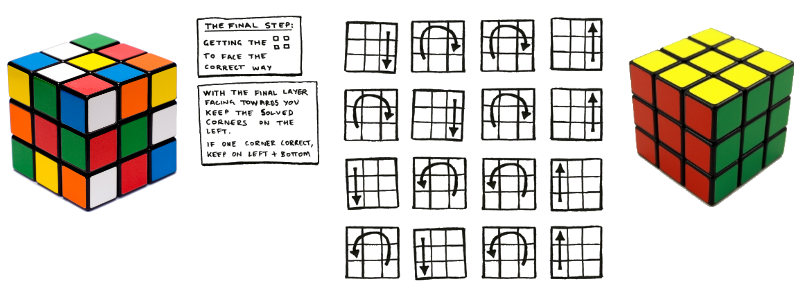
\includegraphics[scale=0.5]{fig/1/Gambar8.png}	
\end{figure}

Salah satu contoh lain yang mewakili algoritma adalah masalah Rubik Cube, jika sebuah Rubik Cube yang belum terselesaikan adalah sebuah masalah dan sebuah Rubik Cube yang sudah selesai adalah solusinya. Maka langkah-langkah penyelesaian yang dilakukan dari masalah menjadi solusi adalah algoritmanya. 

\begin{figure}
	\centering
	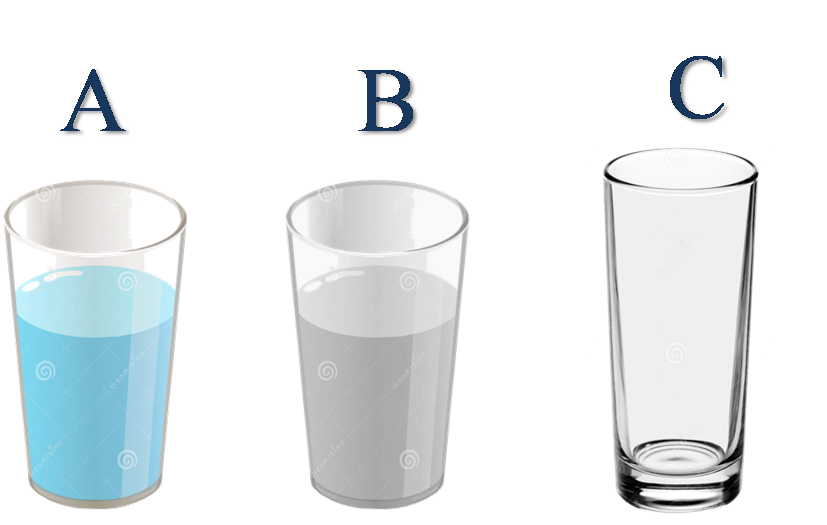
\includegraphics[scale=0.5]{fig/1/Gambar9.png}	
\end{figure}

Perlu diingat, algoritma yang baik adalah algoritma yang terurut dan efektif.  Perhatikan kasus  dimana kita akan memindahkan isi dari gelas A ke gelas B dengan bantuan gelas kosong C, dapatkah Anda menentukan masalah awal, solusi, dan algoritmanya yang efektif ? Bagaimana jika Anda tidak menjalankan algoritmanya tanpa terurut ? 


\subsection{Kenapa harus belajar Algoritma?}
Secara singkat, kita mempelajari algoritma supaya kita bisa menyelesaikan permasalahan-permasalahan komputasional secara \textbf{effisien}\sidenote{Effisien berarti algoritma tersebut memakan waktu dan sumber daya komputasional (mis: memori komputer) yang sedikit}.  

Secara lebih spesifik, tujuan mempelajari algoritma adalah sebagai berikut.
\begin{enumerate}
	\item Dari segi praktikal, kita bisa menyelesaikan berbagai permasalahan yang ada dengan menggunakan sekumpulan algoritma yang sudah tersedia. Sebagai contohnya, jika kita ingin mengurut sejumlah bilangan secara menaik/menurun maka kita bisa menggunakan algoritma pengurutan yang tersedia misalnya \textit{Bubble Sort}, \textit{Merge Sort}, \textit{Quick Sort} dan sebagainya. Selain itu, kita juga bisa merancang algoritma baru yang efisien untuk permasalahan yang lebih spesifik lagi.
	\item Dari segi teoritikal, algoritma merupakan bagian terpenting dari pembelajaran Teknik Informatika/Ilmu Komputer. Pembelajaran algoritma sendiri merupakan inti dari Teknik Informatika dan wajib dipahami oleh mahasiswa sebelum mempelajari mata kuliah tingkat lanjutan.
\end{enumerate}

Sebagai contoh betapa pentingnya algoritma, kita anggap saja ada dua jenis komputer yang berbeda: A dan B. Komputer A adalah komputer yang sangat cepat dan mampu memproses data sebanyak 10 milyar instruksi dalam 1 detik sedangkan komputer B adalah komputer biasa yang hanya mampu memproses data sebanyak 10 juta instruksi dalam 1 detik. Dengan kata lain, komputer A lebih cepat 1000 kali dari komputer B.

\marginnote{Tidak semua permasalahan komputasional bisa diselesaikan secara efisien. Permasalahan yang susah (\textit{Hard Problem}) atau disebut juga permasalahan \textit{NP-complete} masih belum ditemukan algoritma penyelesaian yang effisien.}
Dari contoh sederhana di atas kita bisa menarik kesimpulan bahwa algoritma yang baik bisa mengalahkan algoritma yang buruk sekalipun dijalankan di kondisi yang sangat jelek seandainya masukkannya sangat besar sekali. 
\marginnote{\begin{konsep}
Seandainya ada dua jenis algoritma pengurutan, yaitu: \textit{Insertion Sort} dan \textit{Merge Sort}. \textit{Insertion Sort} memerlukan $8n^2$ langkah sedangkan \textit{Merge Sort} memerlukan $64n \lg n$ untuk masukan $n$. Berapakah nilai $n$ dimana \textit{Insertion Sort} mengalahkan \textit{Merge Sort}?
\end{konsep}
}
Sekarang kita misalkan masing-masing komputer tersebut akan mengurut 10 juta bilangan. Komputer A akan menggunakan algoritma pengurutan X sedangkan komputer B akan menggunakan algoritma pengurutan Y. Algoritma X secara teori tingkat effisiensinya adalah $c_1n^2$ (berarti misalnya untuk setiap 5 bilangan yang diurut, algoritma tersebut memakan waktu $c_15^2 = c_125$ detik, $c_1$ adalah sebuah konstanta yang tergantung pada penerapannya) sedangkan algoritma Y tingkat effisiensinya adalah $c_2n\lg n$. 

Untuk mendramatisir lagi, kita anggap saja algoritma X ditulis oleh programmer yang sangat handal dengan menggunakan bahasa mesin yang sangat effisien sehingga penerapannnya mempunyai tingkat effisiensi $2n^2$ sedangkan algoritma Y ditulis oleh programmer biasa-biasa saja dengan menggunakan bahasa pemrograman yang tidak effisien sehingga penerapannya mempunyai tingkat effisiensi $50n\lg n$.

Sekarang kita bandingkan kedua komputer tersebut ketika mengurut 10 juta bilangan. 
\hspace*{\fill}\\\hspace*{\fill}\\
Komputer A akan memakan waktu:
\hspace*{\fill}\\\hspace*{\fill}\\
$\frac{2\cdot(10^7)^2\ instruksi}{10^{10}\ instruksi/detik} = 20000\ detik\ (5.5\ jam)$
\hspace*{\fill}\\\hspace*{\fill}\\
Sedangkan komputer B akan memakan waktu:
\hspace*{\fill}\\\hspace*{\fill}\\
$\frac{50\cdot10^7lg10^7\ instruksi}{10^{7}\ instruksi/detik} \approx 1163\ detik\ (kurang\ dari\ 20\ menit)$
\hspace*{\fill}\\\hspace*{\fill}\\

\section{Peran Pemrograman pada Algoritma}

Perhatikan salah satu masalah pengurutan voucher yang sudah kita selesaikan sebelumnya. Anggaplah S merupakan himpunan masalah yang akan kita selesaikan dan n merupakan besar / ruang masalah yang akan diselesaikan. Dengan S dan n yang kecil, masalah akan cukup mudah diselesaikan oleh manusia dan dengan cepat. Voucher memiliki $S = \left\langle1,2,3,4,5,6,7,8,9,10\right\rangle$ acak dimana n = 10.

Tetapi bagaimana dengan S yang merupakan himpunan angka acak dari 1 sampai 10.000 $S = \left\langle1,2, ..., 10000\right\rangle$, tentunya dimana n = 10.000 angka. Masalah ini juga bisa diselesaikan oleh manusia, tetapi akan membutuhkan waktu. Dengan perkembangan teknologi saat ini, masalah dengan ruang yang besar dapat diselesaikan oleh kekuatan komputasional (Komputer). Algoritma dapat diterjemahkan menjadi bahasa komputer untuk membantu menyelesaikan masalah. Algoritma dapat diterjemahkan menjadi bahasa komputer melalui pemrograman oleh seorang programmer.  Disinilah hubungannya antara pemrograman dengan algoritma. 


\subsection{Bahasa Pemrograman}
Terdapat banyak bahasa pemrograman dalam Teknik Informatika, kita dapat memilih salah satu yang paling kita sukai dan sesuai dengan tujuan untuk mengakomodasi kita dalam menyelesaikan masalah. Bedasarkan “kemanusiawian”, bahasa pemrograman dikategorikan menjadi dua jenis : 
\begin{enumerate}
	\item \textbf{Low-Level Programming Language}, merupakan bahasa pemrograman yang lebih dekat dengan bahasa mesin. Bahasa pemrograman ini masih berupa instruksi-instruksi yang terkadang tidak memiliki arti dengan bahasa manusia normalnya.Contoh Low-Level Programming Language misalnya : Assembly, OPCODE
	\item \textbf{High-Level Programming Language}, merupakan bahasa-bahasa pemrograman yang dibangun diatas Low-Level Programming Language, namun memiliki bahasa yang lebih masuk akal dan lebih bisa dimengerti karena mengikuti kaidah-kaidah bahasa yang ada. Contoh High-Level Programming Language misalnya	Pascal, Ada, Cobol, Basic, Fortran, C, C++, Python
	\end{enumerate}

Pada mata kuliah ini, kita akan menggunakan bahasa pemrogrman Python. Perlu diingat bahwa, kita bukan mempelajari bahasa pemrograman Python, namun menggunakan Python sebagai alat untuk membantu kita mempelajari penyelesaian masalah melalui pembuatan algoritma dalam bahasa pemrograman.
Tentunya sebagai bahasa pemrograman pertama yang dipelajari, kita perlu tahu bagaimana menginstalasi Python, menggunakan Python dan menjalankan algoritma pertama kita dengan menggunakan Python. Latihan pada bab ini dapat dikerjakan untuk membantu pemahaman penggunaan Python sebelum masuk ke pemahaman algoritma lebih lanjut. 

\chapter{Pengenalan II : Konsep dasar algoritma dan pemrograman}\label{ch:pengantarAlgoritma}

%\section{Konsep dasar algoritma dan pemrograman}

\section{Struktur Dasar Algoritma}
Pada bab sebelumnya, kita mengetahui bahwa Program merupakan kumpulan dari algoritma-algoritma. Algoritma sendiri di dalamnya juga merupakan kumpulan dari struktur-struktur dasar pembangun algoritma. Terdapat tiga jenis utama struktur algoritma yaitu : 

\begin{enumerate}
	\item \textbf{Sequence  (Runtunan)},merupakan struktur algoritma paling dasar yang berisi rangkaian instruksi yang diproses secara sekuensial, satu per satu, mulai dari instruksi pertama sampai instruksi terakhir. Salah satu contoh Sequence(runtunan) ada pada contoh bab sebelumnya yaitu algoritma memindahkan isi dari kedua gelas. 
	\begin{figure}
	\centering
	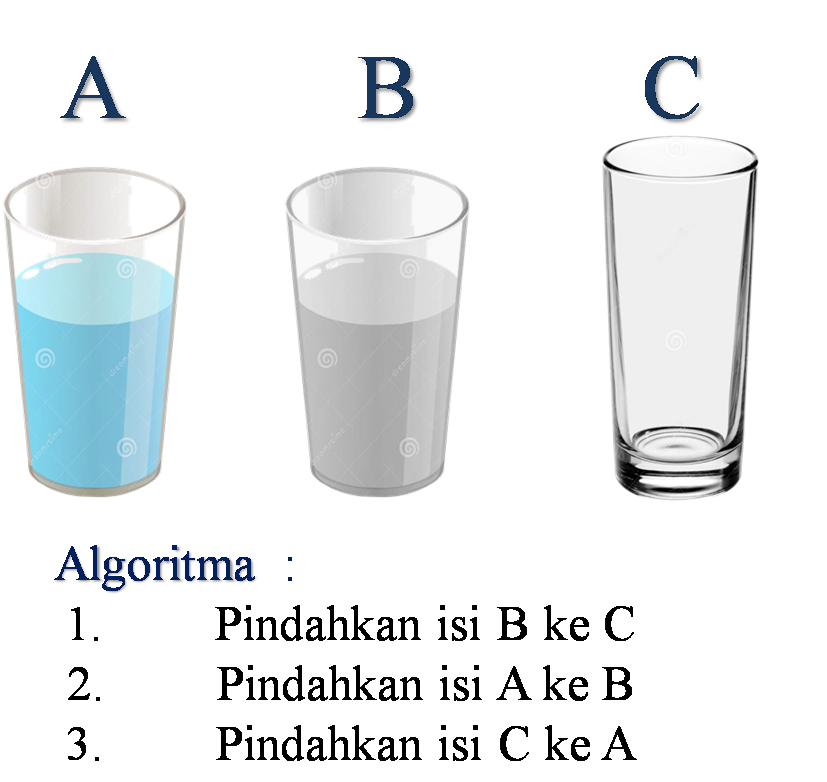
\includegraphics[scale=0.4]{fig/1/Gambar13.png}	
	\end{figure}
	
	\item \textbf{Selection / Branching (Pemilihan / Percabangan)},) merupakan struktur algoritma yang akan digunakan dimana jika terdapat alternatif/pilihan beberapa sequence(runtunan) yang akan dijalankan jika memenuhi syarat tertentu. Percabangan dapat diibaratkan sebagai persimpangan jalan yang harus dipilih, jika kita memilih sebuah jalan dari persimpangan tersebut sudah pasti kita tidak akan menjalani yang lainnya. Salah satu contoh percabangan dapat dilihat pada contoh “Algoritma Memilih Tempat Pembuangan” berikut ini :  
		\begin{figure}
		\centering
		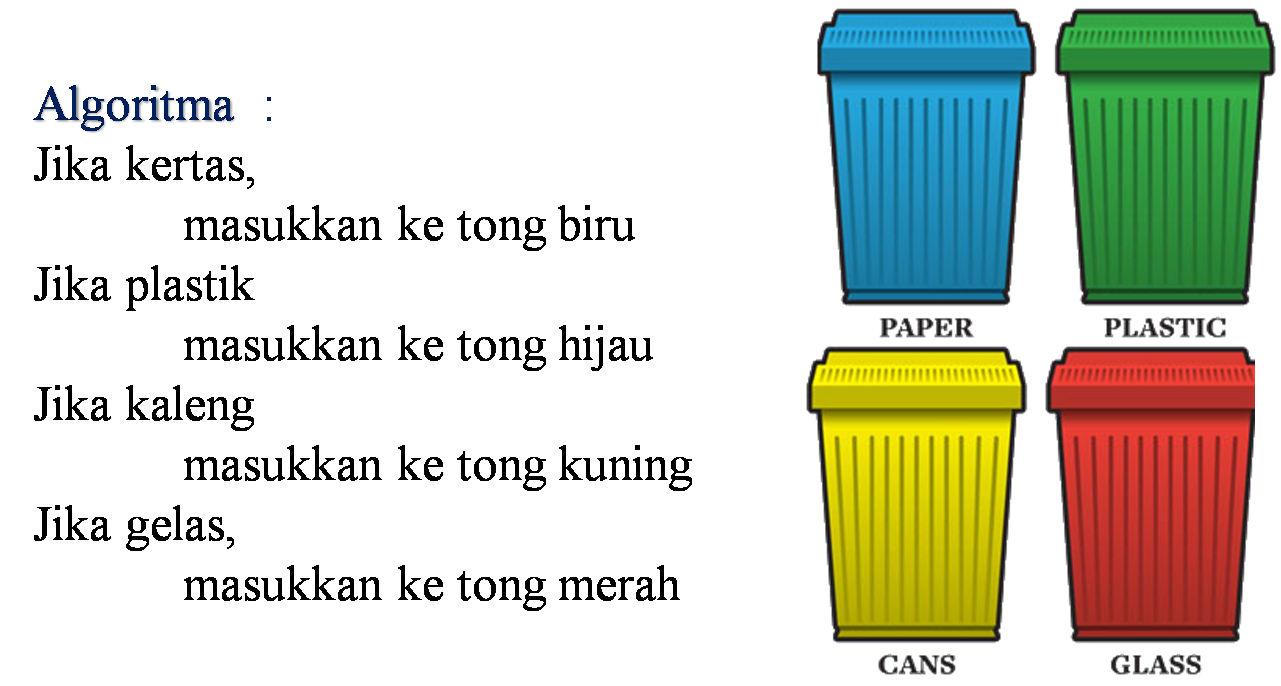
\includegraphics[scale=0.4]{fig/1/Gambar14.png}	
		\end{figure}
		
	\item \textbf{Repetition / Looping (Pengulangan)}, merupakan struktur algoritma yang akan digunakan dimana jika terdapat pengulangan terhadap satu pernyataan atau sequence (runtunan) tertentu. Beberapa contoh nyata penggunaan pengulangan misalnya pada saat harus melakukan penelusuran angka-angka voucher dari awal sampai akhir. Contoh lain yang lebih dekat dengan dunia nyata misalnya adalah algoritma “pembagian permen” berikut ini :
		\begin{figure}
		\centering
		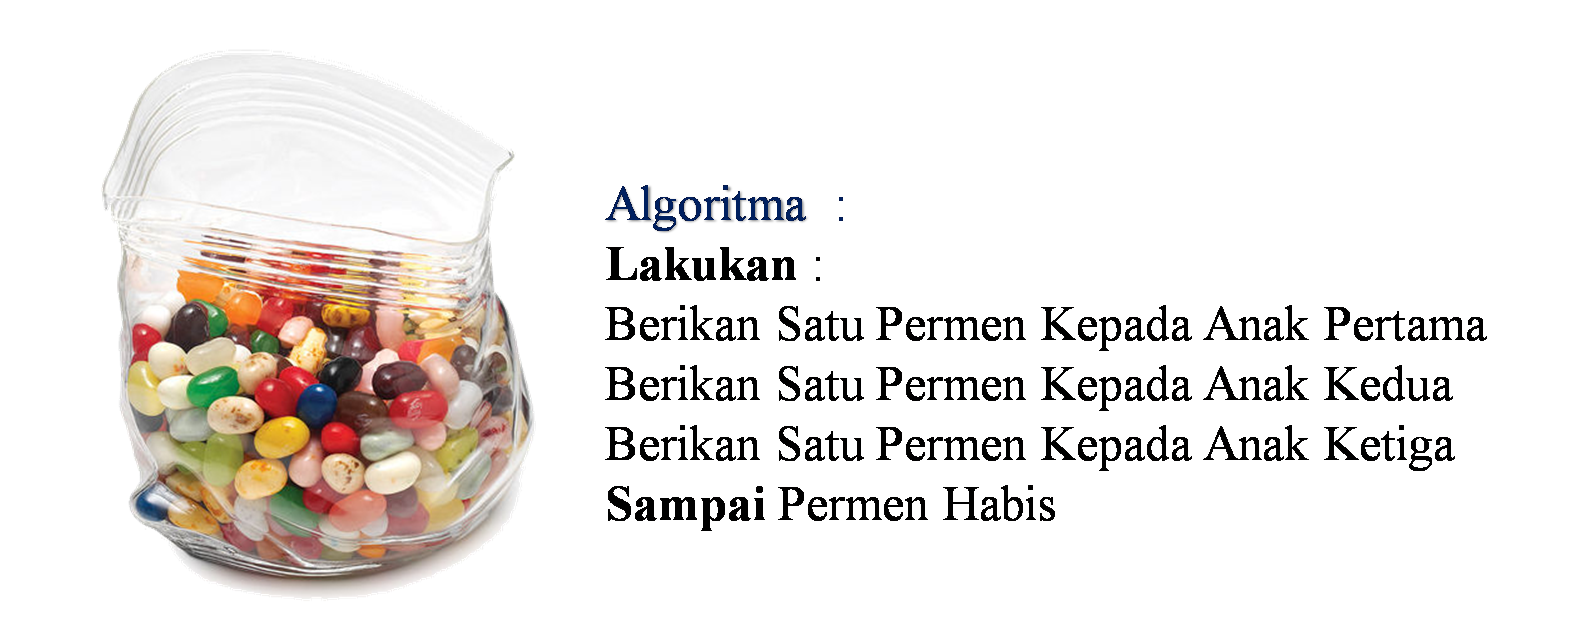
\includegraphics[scale=0.4]{fig/1/Gambar15.png}	
		\end{figure}
\end{enumerate}

Percabangan dan Perulangan akan dibahas lebih lanjut pada pertemuan 3 ke atas. Perlu diperhatikan bahwa masing-masing dari struktur dasar ini tidak berdiri sendiri dan terpisah. Pada kasus pembuatan algoritma sebenarnya, struktur dasar ini akan saling dipasangkan satu sama lain. Beberapa kasus dari penggabungan struktur dasar ini adalah sebagai berikut : 
\begin{itemize}
	\item Perulangan bersarang
	\item	Percabangan bersarang
	\item	Percabangan dalam Percabangan 
	\item	Repetition dalam Percabangan 
	\item	Percabangan dalam Perulangan 
	\item	Perulangan dalam Selection
	\item	Perulangan dalam Perulangan dengan Selection
	\item	Berbagai kombinasi lainnya
\end{itemize}


%\subsection{Tipe Data}
\section{Tipe Data dan Variabel}

\subsection{Tipe Data}
	Dalam mengubah masalah sehari-hari menjadi algoritma, kemudian dari algoritma menjadi bahasa program, kita harus melakukan proses penyederhanaan informasi-informasi dari masalah tersebut. Misalnya, ada masalah menukar isi dalam gelas, kita memerlukan sesuatu yang dapat merepresentasikan / mewakili informasi isi dari gelas seperti sirup atau air  ke dalam algoritma atau bahasa program. Dari sini kita memiliki beberapa alternatif, apakah kita akan mewakilinya dengan kata atau dengan nilai. Dari sinilah muncul konsep tipe-data dalam algoritma. Pada pengenalan akan dikenalkan dahulu beberapa tipe data dasar, kemudian seiring dengan perkembangan mata kuliah, tipe data baru dan yang lebih muktahir akan diperkenalkan. 
Beberapa tipe data dasar yang umum pada algoritma adalah sebagai berikut : 
\begin{itemize}
	\item Bilangan Bulat: Integer, Long
	\item	Bilangan Riil: Float
	\item	Logika : Boolean
	\item	Karakter  : Char
	\item	Kumpulan Karakter : String 
\end{itemize}
Secara umum, tipe data-tipe data inilah yang digunakan untuk mewakiliki kasus-kasus dunia nyata yang akan diterjemahkan menjadi algoritma kemudian menjadi bahasa program. 	


%\subsection{Variabel}
\subsection{Variabel}
Variabel merupakan tempat penyimpanan data. 

Sebagai wadah untuk merepresentasikan dunia nyata pada algoritma, tipe data sendiri tidak cukup. Dengan adanya tipe data saja, maka dalam merepresentasikan masalah kita hanya terbatas pada pembentukan KONSTANTA saja. Misal : “Sirup”, “86.6”, “151”.  Padahal pada kasusnya, informasi-informasi pada masalah sehari-sehari memiliki nilai yang mungkin berubah-ubah. Maka, algoritma juga harus menyediakan wadah untuk menangani hal ini,  disinilah peran VARIABEL dibutuhkan. 
	VARIABEL pada algoritma digunakan untuk menampung nilai dengan tipe data tertentu. Variabel dimaksudkan untuk menyimpan informasi berupa nilai yang dapat secara dinamis berubah, diberi nilainya ataupun dibaca kembali pada saat dibutuhkan. Jika “Sirup” merupakan sebuah nilai dengan tipe data String, dan kita dapat menampungnya dalam sebuah variabel yang bernama GelasA. Yang kita tahu pada kasusnya nanti GelasA akan berubah nilainya ketika ditukar dengan isi dari GelasB.
\begin{contoh}
	\textbf{Penggunaan variabel}\\
	$a = 5 \rightarrow$ Memasukkan nilai 5 ke variabel `$a$'.\\
	$b = 7 \rightarrow$ Memasukkan nilai 7 ke variabel `$b$'.\\
	$a = b \rightarrow$ Memasukkan nilai variabel `$b$' ke variabel `$a$'. Kedua variabel sekarang bernilai 7.\\
	$a = b = 9 \rightarrow$ Memasukkan nilai 9 ke variabel `$a$' dan `$b$'.\\
\end{contoh}

Beberapa peraturan dalam penggunaan variabel adalah sebagai berikut : 
\begin{itemize}
	\item Penamaan variabel sebaiknya eksplisit sesuai dengan tujuan dari pembuatan variabel tersebut. 			  Misalnya : \textit{GelasA} daripada \textit{A}, \textit{GelasB} daripada \textit{B}
	\item	Penamaan variabel tidak boleh melibatkan spasi !  Misalnya : \textit{Gelas A} dan \textit{Gelas B} adalah salah, sedangkan \textit{GelasA} dan \textit{Gelas\underline{ }B} benar
	\item	Penamaan variabel sebaiknya dimulai dengan huruf. Misalnya : \textit{123Panjang} adalah salah. \textit{Panjang123} adalah benar. 
	\item	Pada bahasa pemrograman tertentu, penamaan variabel biasanya case-sensitive. Misalnya : \textit{nama} berbeda dengan \textit{Nama} berbeda dengan \textit{NAMA} berbeda dengan \textit{namA}
	\item	Penamaan variabel jangan bertabrakan dengan reserved-word pada bahasa pemrograman tertentu !
\end{itemize}
Beberapa hal yang akan sering kita lakukan pada pembuatan variabel di algoritma adalah deklarasi dan assignment. Proses inisialisasi awal variabel yang melibatkan pemberian tipe data disebut deklarasi. Proses pemberian nilai pada variabel disebut assigment 

\marginnote[-4cm]{
\begin{konsep}
Jika terdapat 4 variabel, yaitu: a, b, c, dan d dengan nilai a = 1, b = 2, c = 3, dan d =  4. Tuliskan sebuah algoritma untuk menukarkan isi variabel tersebut sehingga nilainya menjadi b = 1, c = 2, d = 3, dan a = 4. Usahakan agar pertukarannya minimum.
\end{konsep}}

%\subsection{Variabel dan Tipe Data Pada Python}
\subsection{Variabel dan Tipe Data Pada Python}
Khusus pada bahasa pemrograman Python, tidak ada deklarasi variabel yang dilibatkan. Pembuatan variabel pada python pada umumnya langsung dibuat melalui proses assignment. Setelah proses assignment, Python akan langsung menyesuaikan tipe data   pada variabel tersebut. Hal ini disebabkan karena Python adalah \textit{dynamically-typed language}. (Istilah optional : Perlu diingat kita bukan mempelajari Python, tetapi Pengantar Algoritma !)
	\begin{figure}
		\centering
		\includegraphics[scale=0.5]{fig/1/Gambar16.png}	
		\end{figure}

\begin{figure}
		\centering
		\includegraphics[scale=0.5]{fig/1/Gambar16a.png}	
		\end{figure}

Perlu diingat juga, peraturan penggunaan variabel sama seperti sub-bab sebelumnya.  Dengan tambahan daftar reserved-words adalah sebagai berikut : 
		\begin{figure}
		\centering
		\includegraphics[scale=0.4]{fig/1/Gambar17.png}	
		\end{figure}



%\subsection{Operator}
\section{Operator}
Pada algoritma, operator berfungsi untuk menghubungkan satu atau lebih variabel sehingga menghasilkan nilai baru. Beberapa operator dasar misalnya adalah sebagai berikut : 

\begin{itemize}

	\item \textbf{Operator Aritmatika}
			\newpage \Large
			\begin{center}
				\begin{tabular}[h!]{| c | c |}
				\hline
				\multicolumn{2}{|c|}{\textit{Operator Aritmatika}} \\
				\hline	
				\textit{Operasi} & \textit{Simbol} & \textit{Python} \\ \hline
				Penambahan & \+ & \\ \hline
				Pengurangan & \- & \\ \hline
				Perkalian & \* & \\ \hline
				Pembagian & \: & \\ \hline
				Perpangkatan & \^ & \\ \hline
				Hasil Sisa Bagi & \% & \\ \hline
				\hline
				\end{tabular}
		\end{center}
		
	
	
	\begin{figure}[h!]
	\centering
	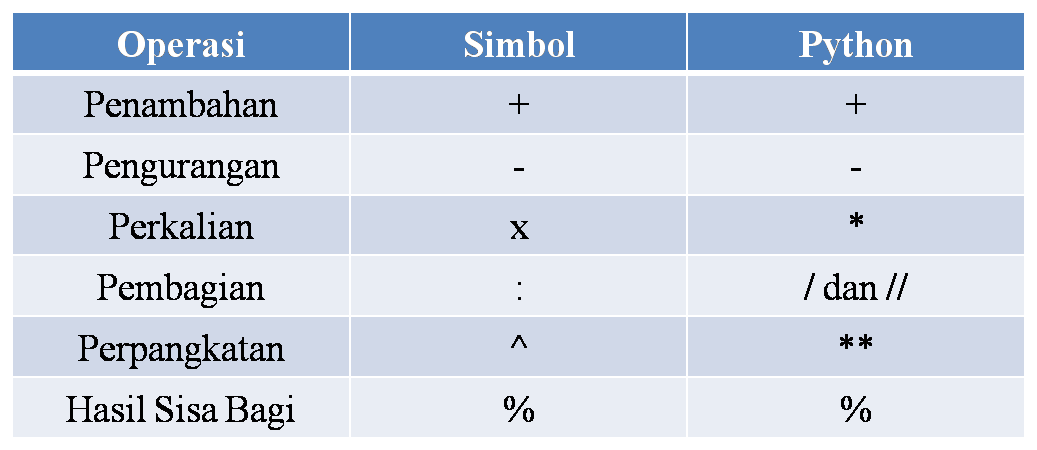
\includegraphics[scale=0.5]{fig/1/Gambar18.png}	
	\end{figure}	

	\item \textbf{Operator Logika}
	\begin{figure}[h!]
	\centering
	\includegraphics[scale=0.5]{fig/1/Gambar19.png}	
	\end{figure}	
	

	\item \textbf{Operator Perbandingan}
	\begin{figure}[h!]
	\centering
	\includegraphics[scale=0.5]{fig/1/Gambar20.png}	
	\end{figure}		
\end{itemize}


 Sama seperti pada matematika dimana pada sebuah perhitungan, operator kali akan dijalankan terlebih dahulu dibanding penambahan dan pengurangan karena memiliki kekuatan operator yang lebih tinggi. 
	\begin{figure}[h!]
	\centering
	\includegraphics[scale=0.5]{fig/1/Gambar21.png}	
	\end{figure}	
Anda boleh mengabaikan operator-operator yang belum diketahui diatas, cukup mengetahui urutan kekuatan operator-operator dasar terlebih dahulu.	

\newpage
\section{Mendefinisikan Permasalahan}
Untuk setiap permasalahan komputasional, ada cara untuk mendefinisikannya. Definisi dibutuhkan untuk menyelesaikan permasalahan tersebut. Definisi dari sebuah permasalahan komputasional bisa dari sangat sederhana seperti di Contoh \ref{cth:pengurutan} sampai ke definisi yang sangat kompleks seperti contohnya permasalahan identifikasi DNA manusia di \textit{Human Genome Project} yang memerlukan algoritma yang sangat kompleks.

Sampai bab ini, kita sudah memiliki pengetahuan yang cukup untuk membuat salah struktur algoritma dasar yaitu sequence(runtunan).  Kembali lagi perlu diingatkan bahwa algoritma dibuat untuk menyelesaikan masalah. Ketika bertemu masalah, agar cara berpikir kita rapi dan efektif, maka alangkah baiknya mengikuti “rule of thumb” berikut ini : 
\begin{enumerate}
	\item Apa masukkan dari masalah ini ? Ini berhubungan dengan bentuk awal dari  masalah. Pertanyaan-pertanyaan ini selanjutnya boleh diperluas dengan memikirkan, berapa variabel yang dibutuhkan di awal? tipe variabel apa saja yang dibutuhkan  di awal ?
	\item Apa keluaran dari masalah ini ? Kapan algoritma akan berhenti ? Apakah algoritma cukup berhenti jika semua proses sudah dijalankan ?  Jika sudah berhenti variabel apa yang akan saya tampilkan kepada pengguna ? Atau bentuk output apa yang akan saya tampilkan kepada pengguna ?  Apakah 
	\item Terakhir, apa proses(algoritma inti) dari masalah ini ? Apakah saya cukup menggunakan runtunan ? Apakah perlu struktur dasar lainnya (Pertemuan berikut !) ? Operator-operator apa saja yang perlu saya gunakan. Perlukah ada variabel-variabel pembantu lainnya ?
\end{enumerate}
Berikut adalah definisi dari permasalahan pengurutan.
\begin{contoh}
\label{cth:pengurutan}
\textbf{Permasalahan Pengurutan (\textit{Sorting Problem})}\\
Diberikan sebuah rangkaian angka $A$, urutkan angka tersebut secara menaik (\textit{ascending}).\\
\textbf{Masukan:}\\
Sebuah rangkaian \textit{n} angka $\left\langle a_{1},a_{2},\ldots,a_{n} \right\rangle$.\\
Misalnya $A = \left\langle 31,41,59,26,41,58 \right\rangle$

\textbf{Keluaran:}\\ 
Permutasi dari \textit{array} angka A $\left\langle a_{1},a_{2},\ldots,a_{n}\right\rangle$ dengan kondisi $\acute{a_{1}} \leq\ \acute{a_{2}} \leq \acute{a_{3}} \ldots \leq \acute{a_{n}}$ \\
Misalnya $A = \left\langle 26,31,41,41,58,59 \right\rangle$
\end{contoh}
Berikut adalah definisi dari permasalahan Pencarian Bilangan Prima.
\begin{contoh}
\label{cth:prima}
\textbf{Permasalahan Pencarian Bilangan Prima}\\
Hasilkan serangkaian bilangan prima dari bilangan $2$ sampai dengan bilangan $n$.\\  
\textbf{Masukan:}\\
Sebuah bilangan bulat \textit{n} yang merupakan batas atas dari \textit{array} bilangan prima yang akan dihasilkan.\\
Misalnya $n = 10$\\
\textbf{Keluaran:}\\
Satu set (himpunan elemen yang tidak memiliki duplikat) bilangan $A$ yang terdiri dari bilangan $2$ sampai bilangan $n$ dimana setiap bilangan hanya memiliki dua pembagi saja yaitu $1$ dan bilangan itu sendiri.\\
Misalnya $A = \left\langle 2,3,5,7 \right\rangle$\\
\end{contoh}
Berikut adalah definisi dari permasalahan Penyebrangan Jembatan.
\begin{contoh}
\textbf{Permasalahan Penyebrangan Jembatan}\\
Ada empat orang yang berusaha menyebrangi sebuah jembatan di malam hari. Karena gelap, mereka membutuhkan sebuah obor untuk menyebrangi jembatan tersebut. Masalahnya adalah obor hanya ada satu dan jembatan tersebut hanya bisa disebrangi oleh dua orang dalam satu waktu yang bersamaan. Setiap orang memiliki waktu yang berbeda ketika menyebrangi jembatan tersebut. Orang pertama memakan waktu 1 menit, orang kedua 2 menit, orang ketiga 5 menit, dan orang keempat 10 menit. 
Agar semua orang bisa menyebrangi jembatan tersebut, maka obor harus dibawa pulang balik ketika melakukan penyebrangan. Hitunglah waktu paling minimal yang diperlukan untuk menyebrangi jembatan tersebut.\\
\textbf{Masukan:}\\
Empat buah bilangan $a,b,c,$ dan $d$ yang masing-masing merepresentasikan waktu yang diperlukan untuk menyebrangi jembatan tersebut untuk setiap orang.\\
Misalnya $a = 1, b = 2, c = 5, d = 10$\\
\textbf{Keluaran:}\\
Sebuah bilangan $z$ dimana bilangan tersebut merupakan waktu minimal yang diperlukan agar keempat orang tersebut berhasil menyebrangi jembatan tersebut.\\
Misalnya $z = 17$\\
\end{contoh}

\subsection{Pseudocode sebagai Notasi Algoritma}
Untuk setiap soal dari contoh-contoh sebelumnya bisa tersedia berbagai macam algoritma yang berbeda untuk menyelesaikannya. Salah satu contoh sederhana dari Contoh \ref{cth:pengurutan} adalah Algoritma \ref{algo:bubble} yang disebut juga dengan nama \textit{Bubble Sort}. 

Algoritma \ref{algo:bubble} ditulis dengan menggunakan pseudocode\sidenote{Pseudocode merupakan sebuah \textit{tool} untuk menuliskan algoritma. Pseudocode bukan merupakan bahasa pemrograman dan tidak bisa dieksekusi.}. Tujuan penggunaan pseudocode adalah agar tidak terikat terhadap bahasa pemrograman tertentu dan bisa lebih fokus ke algoritma saja.

\begin{algorithm}
	\caption{BUBBLE-SORT($A$)}
	\label{algo:bubble}
	\begin{algorithmic}[1]
	\FOR {$i = 1$ \TO $A.length-1$}
		\FOR {$j = i+1$ \TO $A.length$}
			\IF {$A[i] \leq A[j]$}
			\STATE $temp = A[i]$
			\STATE $A[i] = A[j]$
			\STATE $A[j] = temp$
			\ENDIF
		\ENDFOR
	\ENDFOR
	\end{algorithmic}
\end{algorithm}

\marginnote[-4cm]{\begin{konsep}
Berikan beberapa contoh definisi permasalahan komputasional (yang sederhana) yang anda ketahui lengkap dengan masukan dan keluaran dari permasalahan tersebut (min: 3 permasalahan)!
\end{konsep}}

\begin{konsep}
Asumsikan sebuah algoritma menyelesaikan sebuah permasalahan X yang memerlukan $f(n)$ mikrosekon. Untuk setiap $f(n)$ dan waktu $t$ di tabel berikut, tentukan nilai $n$ tertinggi yang bisa diselesaikan dalam waktu $t$.
\begin{figure}%
\centering
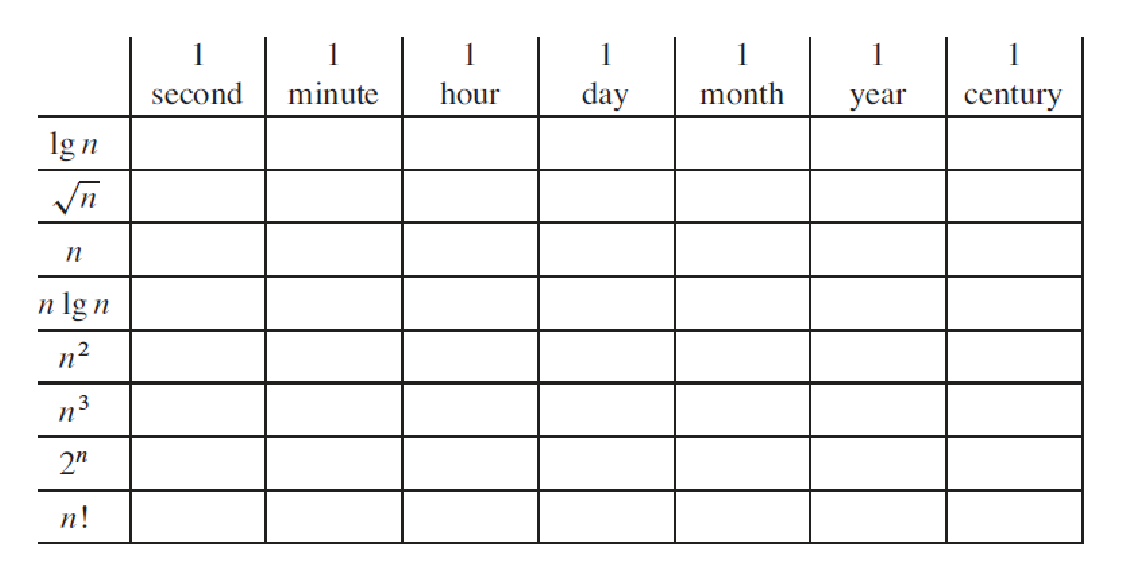
\includegraphics[scale=0.5]{fig/tableEksekusi.eps}%
\end{figure}
\end{konsep}

\subsection{Flow Chart sebagai Notasi Algoritma}
Selain dengan menggunakan pseudocode, bisa juga menggunakan \textit{flow chart} untuk memvisualisasikan sebuah algoritma. Bentuk dari \textit{flow chart} untuk algoritma \ref{algo:bubble} bisa dilihat di gambar \ref{fig:flowchart}.

\begin{marginfigure}%
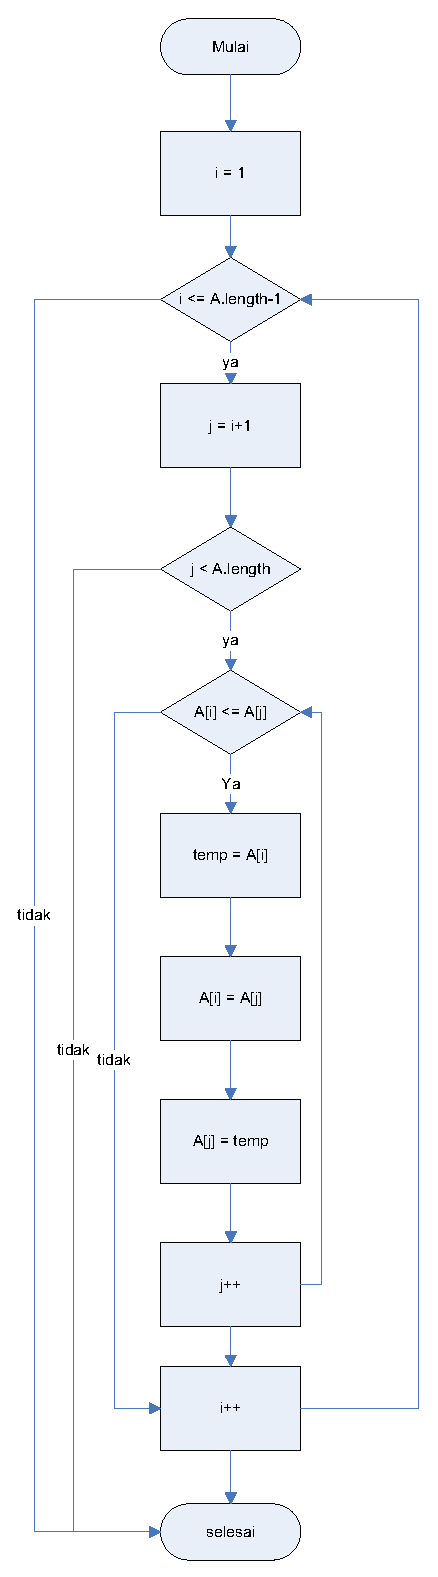
\includegraphics[scale=0.6]{fig/flowchart.eps}%
\caption{Flow Chart Bubble Sort}%
\label{fig:flowchart}%
\end{marginfigure}

\section{Implementasi algoritma ke bahasa pemrograman}
Algoritma \ref{algo:bubble} tidak bisa dijalankan secara langsung tanpa diimplementasi terlebih dahulu ke bahasa pemrograman. Bahasa yang digunakan di Algoritma \ref{algo:bubble} disebut sebagai \textit{pseudocode}. \textit{Pseudocode} sendiri tidak memiliki sebuah standar dalam penulisannya (tidak seperti bahasa Python yang memiliki aturan penulisan/sintaks). Penggunaan \textit{pseudocode} bisa berbeda-beda tergantung pada pembuat/penulisnya. 

Contoh implementasi Algoritma \ref{algo:bubble} ke bahasa pemrograman (Python) bisa dilihat di Listing \ref{lst:bubbleSortSimple}. Perlu diketahui, terdapat beberapa perbedaan mendasar antara algoritma dan listing program (misalnya indeks di algoritma dimulai dari 1 sedangkan di bahasa Python dimulai dari 0). 

\begin{listprog}{bubbleSort.py}
	\label{lst:bubbleSortSimple}
	\begin{lstlisting}[language=Python]
		A = [4,1,3,5,6,7,2]
		for i in range(1,len(A)):
				for j in range(i+1):
						if A[i]<=A[j]:
								temp = A[i]
								A[i] = A[j]
								A[j] = temp
		print A
	\end{lstlisting}
\end{listprog}

		
%\FloatBarrier
%\subsection{Array}
%Array\sidenote{Di bahasa pemrograman Python, implementasi dari Array disebut sebagai List.} merupakan kumpulan dari variabel. Satu array bisa menampung beberapa data. Gambar \ref{fig:illustrasiArray} menunjukkan illustrasi dari sebuah array yang berkapasitas $j$.
%\begin{center}
	%\begin{figure}[htbp]%
		%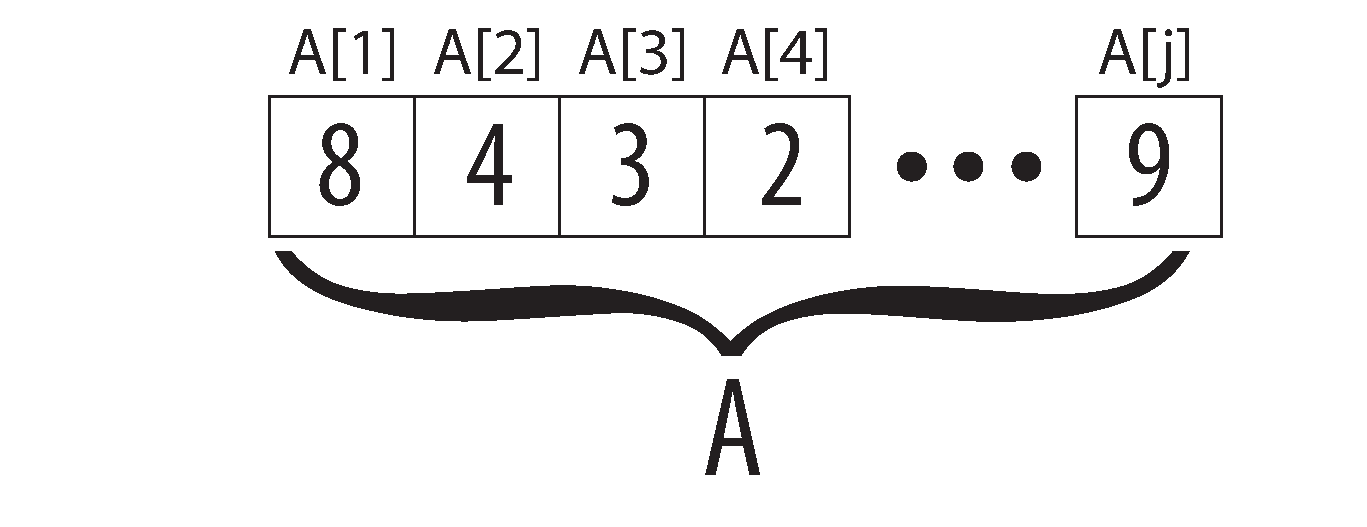
\includegraphics[scale=0.4]{fig/Array.eps}%
		%\caption{Illustrasi Array}%
		%\label{fig:illustrasiArray}%
	%\end{figure}
%\end{center}
%\begin{contoh}
	%\textbf{Penggunaan array}\\
	%$A[i] \rightarrow$ Mengakses lokasi ke $i$ dari array yang bernama $A$.\\
	%$A[4] \rightarrow$ Mengakses lokasi ke $4$ dari array yang bernama $A$.\\
	%$A[i..j] \rightarrow$ Menandakan kumpulan isi array $A$ yang terdiri dari elemen $A[1],\ A[2],\ A[3],\ \ldots,\ A[j]$.\\
	%$A[4] = 5 \rightarrow$ Memasukkan nilai 5 ke lokasi ke 4 dari array $A$.\\
	%$b = A[4] \rightarrow$ Memasukkan nilai lokasi ke 4 dari array $A$ ke variabel $b$. 
	%$A.length \rightarrow$ Menandakan besar/panjang dari array $A$.
%\end{contoh}

\begin{pemrograman}
Lakukan langkah-langkah berikut di rumah:
\begin{enumerate}
	\item Unduh Python di \url{http://python.org/download/}.
	\item Pilihlah python versi 2.7.x yang sesuai dengan OS yang dipakai (Windows 32-bit---Python 2.7.3 Windows Installer, dan Windows 64-bit---Python 2.7.3 Windows Installer). Untuk Linux, python sudah secara \textit{default} terinstall (versi python tergantung dari distro linux yang digunakan).
	\item Install Python Installer yang sudah diunduh.
	\item Unduh IDE \textit{Integrated Development Environment} Python yang bernama PyScripter di \url{http://code.google.com/p/pyscripter}.
	\item Install PyScripter.
	\item Ketikkan Listing \ref{lst:bubbleSortSimple} dan jalankan.
\end{enumerate}
\end{pemrograman}

\begin{pemrograman}
Untuk melakukan latihan pemrograman algoritma dan Python di rumah, SPOJ merupakan website yang sangat berguna. SPOJ merupakan sebuah website \textit{Online Judge} dimana kita bisa melihat permasalahan-permasalahan yang menarik, menyelesaikan permasalahan tersebut dan meng-\textit{submit} solusinya ke SPOJ untuk di-\textit{judge}. SPOJ akan menentukan apakah solusi kita tepat atau salah. Diharapakan agar mahasiswa bisa menyelesaikan permasalahan SPOJ sebanyak mungkin untuk meningkatkan kemampuan pemrograman. Berikut langkah-langkah yang harus dilakukan di rumah.
\begin{enumerate}
	\item Buka website SPOJ (\url{www.spoj.pl})
	\item Register di website SPOJ tersebut.
	\item Baca tutorial di website SPOJ untuk memahami lebih lanjut di \url{http://www.spoj.pl/tutorials/}
	\item Lihat daftar permasalahan (\textit{problems}) di website SPOJ di \url{http://www.spoj.pl/problems/classical}
	\item Lihat permasalahan yang paling sederhana, yaitu permasalahan nomor 1 dengan CODE ``TEST'', atau dengan nama ``Life, the Universe, and Everything'' (\url{http://www.spoj.pl/problems/TEST/}).
	\item Baca dan coba pahami soalnya.
	\item Untuk percobaan akan dikasihkan solusinya sebagai berikut dalam bentuk \textit{source code} Python. 
	\begin{listprog}{TEST.py}
	\label{lst:TEST}
	\begin{lstlisting}[language=Python]
		k=input()
		while k!=42:
			print k
		k=input()
	\end{lstlisting}
	\end{listprog}
	\item Submit solusi tersebut di \url{http://www.spoj.pl/submit/}, pastikan pilihan \textbf{Language} adalah Python (python 2.7) dan Problem code adalah TEST.
	\item Lihat hasilnya di \url{http://www.spoj.pl/status/} dan cari username anda di kolom USER. Jika ada tulisan ``accepted'' berarti anda telah berhasil menyelesaikan permasalahan tersebut. Jika tidak cek kembali apakah ada yang salah di langkah sebelumnya.
\end{enumerate}
\end{pemrograman}
